\documentclass[12pt]{article}
\setlength\parindent{0pt}
\usepackage{fullpage}
\usepackage{amsmath}
\usepackage[dvipsnames]{xcolor}
\usepackage{graphicx}
\usepackage{tikz}
\setlength{\parskip}{4mm}
\usepackage[left=2cm, right=2cm, top=1.5cm, bottom=1cm]{geometry}
%\usepackage[margin=0.5in, paperwidth=13.5in, paperheight=8.4375in]{geometry}
\def\LL{\left\langle}   % left angle bracket
\def\RR{\right\rangle}  % right angle bracket
\def\LP{\left(}         % left parenthesis
\def\RP{\right)}        % right parenthesis
\def\LB{\left\{}        % left curly bracket
\def\RB{\right\}}       % right curly bracket
\def\PAR#1#2{ {{\partial #1}\over{\partial #2}} }
\def\PARTWO#1#2{ {{\partial^2 #1}\over{\partial #2}^2} }
\def\PARTWOMIX#1#2#3{ {{\partial^2 #1}\over{\partial #2 \partial #3}} }
\newcommand{\BI}{\begin{itemize}}
\newcommand{\EI}{\end{itemize}}
\newcommand{\BE}{\begin{displaymath}}
\newcommand{\EE}{\end{displaymath}}
\newcommand{\BNE}{\begin{equation}}
\newcommand{\ENE}{\end{equation}}
\newcommand{\BEA}{\begin{eqnarray}}
\newcommand{\EEA}{\nonumber\end{eqnarray}}
\newcommand{\EL}{\nonumber\\}
\newcommand{\la}[1]{\label{#1}}
\newcommand{\ie}{{\em i.e.\ }}
\newcommand{\eg}{{\em e.\,g.\ }}
\newcommand{\cf}{cf.\ }
\newcommand{\etc}{etc.\ }
\newcommand{\Tr}{{\rm tr}}
\newcommand{\etal}{{\it et al.}}
\newcommand{\OL}[1]{\overline{#1}\ } % overline
\newcommand{\OLL}[1]{\overline{\overline{#1}}\ } % double overline
\newcommand{\OON}{\frac{1}{N}} % "one over N"
\newcommand{\OOX}[1]{\frac{1}{#1}} % "one over X"

\def\BS{\bigskip}

\begin{document}
\pagenumbering{gobble}
\Large
\centerline{\sc{Recitation Questions -- 1D Motion (part 1)}}
\normalsize
\centerline{\sc{Week 1, Day 2}}
\normalsize
\medskip

\BS\BS\BS


In this recitation, you will learn how to:

\BI
\item describe simple motions in words, pictures, and mathematics, and relate those descriptions to each other
\item construct algebraic representations of questions about motion
\item think carefully about how position, velocity, and acceleration relate
\EI


{\color{Red}A note -- Question 4 is challenging! You may wish to have students skip Question 3, do Question 4, then come back to Question 3 if time permits. That's up to you!}

\centerline{\Large Question 1: Two runners}

\begin{center}
\it (This problem is simple, but it has the same template as most of the problems that you'll be doing for this unit. Take note of the steps you take to solve it; the steps will be similar for very many of the things you do in the next few weeks.)

\end{center}
\rm
Two runners, Alice and Bob, start at opposite ends of a hundred-meter long soccer pitch and sprint toward each other. Alice runs at 8 m/s and starts on the east side, while Bob runs at 6 m/s and starts at the west side. You'd like to know where they'll meet.


\begin{enumerate}

\item Draw position vs. time graphs for both runners on a single set of axes.

\begin{center}

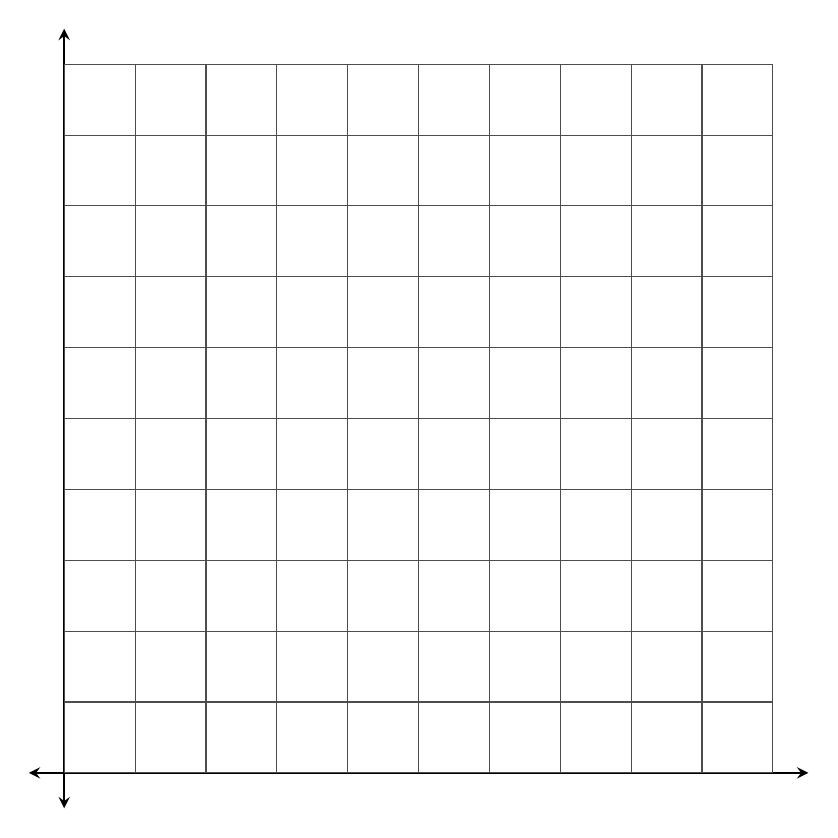
\begin{tikzpicture}[scale=0.9]
\pgfmathsetmacro{\xmin}{0}
\pgfmathsetmacro{\xmax}{10}
\pgfmathsetmacro{\ymin}{0}
\pgfmathsetmacro{\ymax}{10}

\coordinate (o) at (0,0);

\draw[thick,stealth-] (\xmin,0) +(-0.5,0) -- (\xmax,0);
\draw[thick,-stealth] (\xmax,0) -- +(0.5,0);
\draw[thick,stealth-] (0,\ymin) +(0,-0.5) -- (0,\ymax);
\draw[thick,-stealth] (0,\ymax) -- +(0,0.5);

\draw[black!70] (\xmin,\ymin) grid (\xmax, \ymax);

\end{tikzpicture}




\end{center}

{\color{Red} It is deliberately left up to the student whether ``up" on the graph will be east or west (or, alternatively,
	which one starts on the bottom and which starts on the bottom). Students will need to choose a coordinate system. Either choice is fine. They will also need to realize that ``toward each other'' means that the lines representing their motion should move toward one another.}


\item Write position vs. time equations for both runners. Since they are running at constant velocity, their equation of motion will be $x=x_0 + vt$. However, in this case you've got two different $x$'s and two different $v$'s. Use subscripts to distinguish their positions, \ie $x_A$ and $x_B$. Hint: Think carefully about their velocities...

{\color{Red} Here we are getting them used to translating between descriptions of motion in words, algebraic representations (equations of motion), and graphical representations. They'll need to recognize that one of them starts at $x=0$ and has a positive velocity, and the other starts at $x=100$ and has negative velocity. Think about what you'd say to a student who writes both velocities as positive -- this is one of the biggest errors they make here.}

\vspace{1.5in}

\item In this entire unit, the main challenge will be translating the question (``where will they meet?'') into a sentence that involves your algebraic variables. This sentence will then become your recipe for solving the problem.
Often, but not always, this will take the following form: 

\begin{center}
{\bf ``What is the value of \underline{\hspace{0.7in}} at the time when \underline{\hspace{0.7in}} is equal to \underline{\hspace{0.7in}}?''} 
\end{center}

Fill in the blanks in the above sentence to get a recipe for figuring out where the runners will meet.

{\color{Red} \bf We are going to be doing a ton of this in the first unit. \rm It's my experience that students who have trouble with kinematics most often mess up this step: translating ``what you're trying to do'' into symbols. Many students will find this trivial; this is a warmup for 2D motion when it is not always so trivial. So we're practicing the process now. They should find the value of $x_1$ or $x_2$ at the time when $x_1$ is equal to $x_2$.}

\item Do the algebra indicated by your recipe and figure out where they will meet.

{\color{Red}If they did what we suggested above and wrote out the sentence -- ``What is the value of $x_1$ at the time when $x_1 = x_2$'' -- it should be very clear what to do.}


\item Suppose that instead Bob had a 2 second head start. What would change in your graphs? What would change in your algebra? (Discuss this in words and symbols; you don't need to do the arithmetic again.)

{\color{Red} Here they need to fiddle with the time variables. There are a lot of approaches they could take here. One is to use two separate time variables ($t_a$ and $t_b$), then relate the two. Another is to do this in one step, think about what moment $t=0$ represents (probably the moment that Bob starts running), and then replace $t$ with $t-2$ in Alice's equation of motion. This exercise is here to prompt students to think carefully about what their variables mean: ``what does $t$ represent? The time since which moment? What is happening at $t=0$?''}


\end{enumerate}


\vspace{3in}
\newpage
\centerline{\Large Question 2: Motion with acceleration}

In class, you learned the kinematics relations

\begin{align*}
x(t) &= x_0 + v_0t + \frac{1}{2}at^2 \\
v(t) &= v_0 + at
\end{align*}

These relations aren't generally true, however; they are true only in a specific case. What must be true about the object's acceleration for these relations to apply? {\it (You don't need to calculate anything here; this is something you should remember from class.)}

\vspace{1.2in}

{\color{Red}
This applies only if acceleration is constant. This is important for them to keep in mind when we talk about regimes of validity and motion where the acceleration is only piecewise constant.}
\newpage






\centerline{\Large Question 3: a braking car}

A car is traveling at 30 m/s and applies its brakes to slow down to 10 m/s. If it is able to decelerate at 5 $\rm m/\rm s^2$, how far does it travel during the braking period?

\begin{enumerate}
	\item Write expressions for the car's position and velocity as a function of time. What moment makes sense to choose as your reference time $t=0$?
	
	\vspace{1in}
{\color{Red} Here, they need to interpret the word ``decelerate'' to mean ``accelerate in a direction opposite its motion'' -- i.e., if $v_0$ is positive, $a$ is negative. The moment when the car first applies its brakes is the obvious choice for $t=0$ (the moment when the acceleration begins).}
	
	\item How can you translate the question ``How far does it travel during the braking period?'' into a sentence about your algebraic variables? Again, fill in the blanks: 
	
	\begin{center}
		{\bf ``What is the value of \underline{\hspace{0.7in}} at the time when \underline{\hspace{0.7in}} is equal to \underline{\hspace{0.7in}}?''} 
	\end{center}
	{\color{Red} Here, again, we are practicing this while it is easy; it will get harder later. Assuming $x=0$ is also the position when the car applies its brakes, we want ``What is the value of position at the time that $v=10$ m/s?''}
	
	\item What intermediate quantity must you find before you find the distance traveled? Following the above recipe you created for yourself, find it.
	
	{\color{Red} This is the time. They'll need to go to the velocity equation to find that the braking time is 4 seconds.}
	

	
	
	\vspace{2in}
	
	
	
	
	
	\item Finally, how far does the car travel during the braking period?
	
	{\color{Red}Here they should recognize that they their sentence above -- ``What is the value of position at the time that $v=10$ m/s?'' -- gives them a roadmap for what to do: now that they have found the time that $v=10$ m/s, they should find the position at that time by substituting this time into their position equation.
	
Their position equation is 

$$x(t) = v_0 t + \frac{1}{2}at^2$$

Substituting in numbers we get:

$$x(t) = (30\, \rm m/\rm s) (4 s) - \frac{1}{2}(-5\, \rm m/\rm s^2)(4 s)^2 = 120 m - 40 m = 80 m$$}
	
	\newpage


\centerline{\Large Question 4: A bouncing basketball}

\BS

{\color{Red}THIS QUESTION IS CHALLENGING. Part of why it is here is to encourage a bit of humility among students who have taken AP Physics and think the initial portion of this class will be a breeze. It is fine if you have students skip Question 3, do this one, and then go back to Question 3 if time permits. They will benefit from doing this in larger groups at the chalkboard (perhaps two groups around one set of graphs -- 6 people total).}

A person is holding a basketball; they drop the basketball (from rest). It falls to the ground, bounces back up, and falls back down again. Draw position vs. time, velocity vs. time, and acceleration vs. time graphs for the ball on the next page. Alternatively, several groups can work on this together by drawing their graphs on the board and discussing them as a large group.

Look at your graphs carefully and make sure they are self-consistent:


\BI
\item Regions of constant acceleration should correspond to places where the velocity graph is a straight line (are there any regions where the acceleration is constant? Are there any regions where it is something different?)
\item Regions of constant velocity should correspond to places where the position graph is a straight line (are there any?)
\item Places where the position graph is flat should correspond to $v=0$. (are there any?)
\item Remember, the slope of the position graph is the value of the velocity graph; the slope of the velocity graph is the value of the acceleration graph. This means:
\begin{itemize}
	\item If the velocity is positive, the position graph should be going up
	\item If the velocity is negative, the position graph should be going down
	\item If the acceleration is positive, the velocity should be going up, and the position graph should be concave upwards
	\item If the acceleration is negative, the velocity should be going down, and the position graph should be concave downwards
\end{itemize}
\EI


Note: This can be surprisingly tricky and will provoke a fair amount of debate among your peers -- this is what we intend for you to do! As with all problems in recitation, work together with your peers and ask your TA/coach for guidance if you have questions.

\BS\BS

{\it Hint:} There is some tension here between the ``engineering reality'' of how a basketball really bounces -- where it's in contact with the ground for a measurable amount of time, during which it bounces back upward
-- and a mathematical idealization of it. You should think about a {\it real} basketball bouncing on a {\it real} floor.

\newpage


\begin{center}
	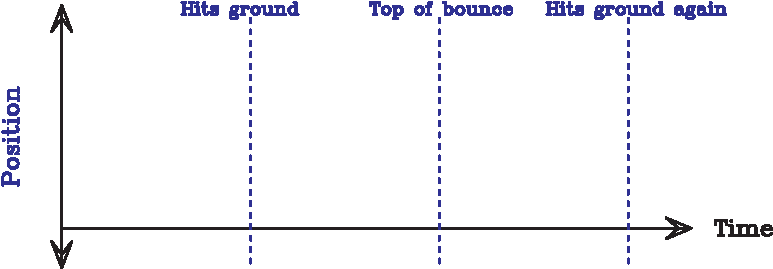
\includegraphics[width=\textwidth]{position-crop.pdf}
	
	\vspace{0.4in}
	
	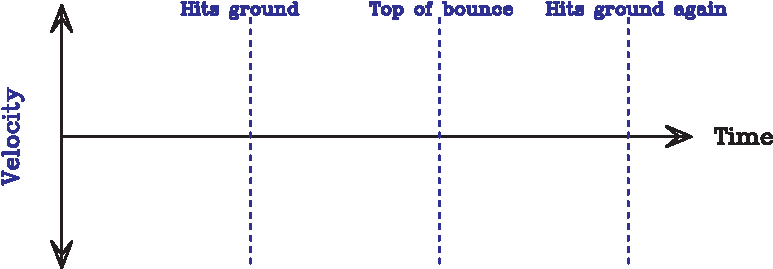
\includegraphics[width=\textwidth]{velocity-crop.pdf}
	
	\vspace{0.4in}
	
	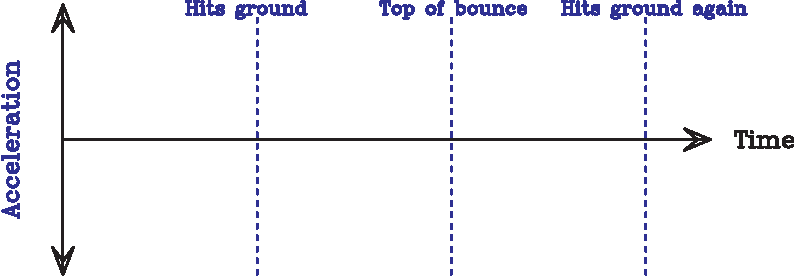
\includegraphics[width=\textwidth]{acceleration-crop.pdf}
\end{center}

{\color{Red}
	The challenge here is figuring out what happens at the bounce point. They may start with any of the three graphs first -- position, velocity, or acceleration -- although it is probably easiest to start with velocity. 
	
	Students' progress through this question generally involves them starting with one of the three graphs, then trying to draw the others in ways that are consistent both with the description of the motion and with the requirement that the velocity is the slope of position and that acceleration is the slope of velocity. (This means, for instance, that since the ball is in freefall everywhere except when it is in contact with the ground, acceleration is -g everywhere except at that point, and that the velocity line must have a uniform negative slope everywhere except at that point.)
	
	When teaching this, the best way to help students is to ask about inconsistencies in what they do -- ask them to explain why they've done what they've done, ask why they've drawn the graphs in the shapes that they have, and ask what the shape of one graph implies about the others.
	
	They should figure out that the velocity starts at zero and decreases linearly during the initial fall to the ground. Then, when it bounces, the velocity rapidly changes from a large negative value to a large positive value. Then it decreases linearly again, reaching zero at the point when the ball is highest off the ground and becoming negative as the ball falls back down again.
	
	What about acceleration? They will need to recognize that the acceleration {\it does not do anything special} at the point when the ball reaches its apex on the bounce; it is in free fall whether it is going up or going down. Only at the moment when the ball is actually touching the ground does the acceleration change -- for that moment only, it is a large positive spike (while the floor is pushing it upward). 
	
	Finally, they can figure out the position graph from the velocity one -- it is always a concave down parabola, with a cusp when it bounces. You should ask them if they've finished Calc 1 -- if they have you can talk about concavity; otherwise, you should encourage them to say things like ``well, if the velocity starts at zero and becomes more negative, then the position graph should start flat and then curve more and more downward, since velocity is the slope of position and it is becoming more negative. And then after it bounces, it goes back up, but its slope becomes less and less positive as velocity gets closer and closer to zero...'' -- essentially, you are teaching them about concavity without using the word.
}
	




\end{enumerate}

\end{document}
